\chapter{Non-parametric DF Estimation}
So far, we have been interested in some estimation problems involved in parametric experiments.  In parametric experiments, the parameter space $\BB{\Theta}$ can have many dimensions, but these are finite.  For example, in the $n$ IID $\bernoulli(\theta^*)$ and the $n$ IID $\exponential(\lambda^*)$ experiments:
\begin{eqnarray*}
X_1,\ldots,X_n \overset{IID}{\sim} \bernoulli(\theta^*), & \qquad & \theta^* \in \BB{\Theta}=[0,1] \subset \Rz^1 \enspace , \\
X_1,\ldots,X_n \overset{IID}{\sim} \exponential(\lambda^*), & \qquad & \lambda^* \in \BB{\Lambda}=(0,\infty) \subset \Rz^1 \enspace ,
\end{eqnarray*}
the parameter spaces $\BB{\Theta}$ and $\BB{\Lambda}$ are of dimension $1$.  Similarly, in the $n$ IID $\normal(\mu,{\sigma}^2)$ and the $n$ IID $\lognormal(\lambda,\zeta)$, experiments:
\begin{eqnarray*}
X_1,\ldots,X_n \overset{IID}{\sim} \normal(\mu,\sigma^2), &\qquad & (\mu,\sigma^2) \in \BB{\Theta}=(-\infty,+\infty) \times (0,+\infty) \subset \Rz^2 \\
X_1,\ldots,X_n \overset{IID}{\sim} \lognormal(\lambda,\zeta), &\qquad & (\lambda,\zeta) \in \BB{\Theta}=(0,+\infty) \times (0,+\infty) \subset \Rz^2 
\end{eqnarray*}
the parameter space is of dimension $2$.

An experiment with an infinite dimensional parameter space $\BB{\Theta}$ is said to be {\bf non-parametric} .  Next we consider a non-parametric experiment in which $n$ IID samples are drawn according to some fixed and possibly unknown DF $F^*$ from the space of {\bf All Distribution Functions}:
\[
\boxed{
X_1,X_2,\ldots,X_n \overset{IID}{\sim} F^*, \qquad F^* \in \BB{\Theta} = \{ \text{All DFs}\} := \{ \,  F(x; F) :  F~is~a~DF \, \} 
}
\]
where the DF $F(x; F)$ is indexed or parameterised by itself. Thus, the parameter space $\BB{\Theta}=\{ \text{All DFs}\}$ is the {\bf infinite dimensional} space of {\bf All DFs}.  In this section, we look at estimation problems in non-parametric experiments with an infinite dimensional parameter space.  That is, we want to estimate the DF $F^*$ from which our IID data are drawn.

The next proposition is often referred to as the {\bf fundamental theorem of statistics} and is at the heart of non-parametric inference, empirical processes, and computationally intensive bootstrap techniques.  Recall  \hyperref[D:ECDF]{Definition~\ref*{D:ECDF}} of the $n$-sample empirical distribution function (EDF or ECDF) $\widehat{F}_n$ that assigns a probability mass of $1/n$ at each data point $x_i$:
\begin{eqnarray*} %\label{E:ECDF}
\widehat{F}_n(x) = \frac{ \sum_{i=1}^n \BB{1}(X_i \leq x) }{n} \ ,  & \quad where \qquad
\BB{1}(X_i \leq x) :=
\begin{cases}
& 1  \quad \text{if $x_i \leq x$} \\
& 0  \quad \text{if $x_i > x$} 
\end{cases}
\end{eqnarray*}

\begin{figure}[htpb]
\caption{Plots of ten distinct ECDFs $\widehat{F}_n$ based on $10$ sets of $n$ IID samples from $\uniform(0,1)$ RV $X$, as $n$ increases from $10$ to $100$ to $1000$.  The DF $F(x)=x$ over $[0,1]$ is shown in red.  The script of \hyperref[Mf:GilvenkoCantelliUnif01n10n100n100ECDFs]{Labwork \ref*{Mf:GilvenkoCantelliUnif01n10n100n100ECDFs}} was used to generate this plot.   \label{F:GilvenkoCantelliUnif01n10n100n100ECDFs}}
\centering   \makebox{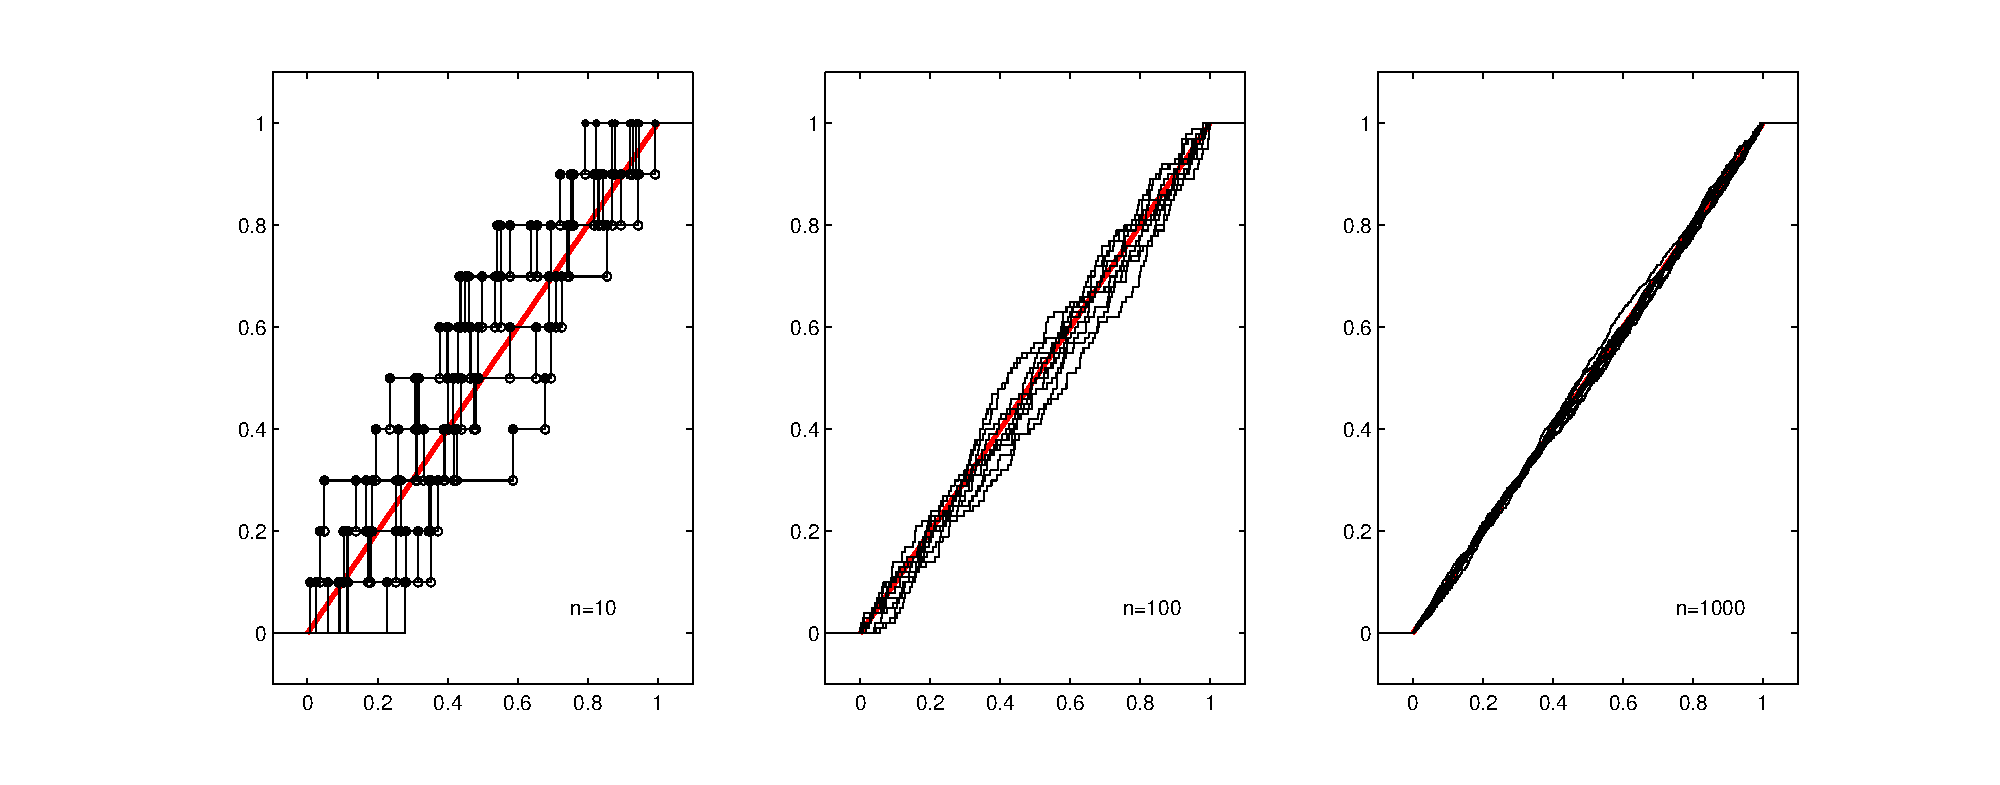
\includegraphics[width=6.50in]{figures/GilvenkoCantelliUnif01n10n100n100ECDFs}}
\end{figure}
\begin{prop}[Gilvenko-Cantelli Theorem]\label{P:Gilvenko-Cantelli}
Let $X_1,X_2,\ldots,X_n \overset{\IID}{\sim} F^*$.  Then:
\[
\sup_x { | \widehat{F}_n(x) - F^*(x) | } \overset{P}{\longrightarrow} 0 \ .
\]
%{\scriptsize
%\begin{proof}
%Proof to be seen in STAT 318 or another advanced Statistics course.
%\end{proof}
%}
\end{prop}
{\bf Heuristic Interpretation of the Gilvenko-Cantelli Theorem}:  As the sample size $n$ increases, the empirical distribution function $\widehat{F}_n$ converges to the true DF $F^*$ in probability, as shown in \hyperref[F:GilvenkoCantelliUnif01n10n100n100ECDFs]{Figure~\ref*{F:GilvenkoCantelliUnif01n10n100n100ECDFs}}.

\begin{prop}[The Dvoretzky-Kiefer-Wolfowitz (DKW) Inequality]
Let $X_1,X_2,\ldots,X_n \overset{\IID}{\sim} F^*$.  Then, for any $\epsilon>0$:
\begin{equation}\label{E:DKWNeq}
P \left( \sup_x | \widehat{F}_n(x) - F^*(x) | > \epsilon  \right) \leq 2 \exp {(-2 n \epsilon^2)}
\end{equation}
Recall that $\sup(A)$ or supremum of a set $A \subset \Rz$ is the least upper bound of every element in $A$.
\end{prop}

\section{Estimating DF}\label{S:EstimDF}
Let $X_1,X_2,\ldots,X_n \overset{\IID}{\sim} F^*$, where $F^*$ is some particular DF in the space of all possible DFs, i.e.~the experiment is non-parametric.  Then, based on the data sequence $X_1,X_2,\ldots,X_n$ we want to estimate $F^*$.

For any fixed value of $x$, the expectation and variance of the empirical DF \eqref{E:ECDF} are:
\begin{eqnarray}
\e \left( \widehat{F}_n(x) \right) &=& F^*(x) \implies \mathsf{bias}_n \left( \widehat{F}_n(x) \right) = 0 \label{E:FnhatUnbiased} \\
\V \left( \widehat{F}_n(x) \right) &=& \frac{F^*(x) (1-F^*(x))}{n} \implies \lim_{n \to \infty}\mathsf{se}_n \left( \widehat{F}_n(x) \right) = 0  \label{E:Fnhatseto0} 
\end{eqnarray}
Therefore, by \hyperref[P:AsympConsistencyUnbiasedSE0]{Proposition~\ref* {P:AsympConsistencyUnbiasedSE0}}, the empirical DF evaluated at $x$, i.e.~$\widehat{F}_n(x)$ is an asymptotically consistent estimator of the DF evaluated at $x$, i.e.~$F^*(x)$.  More formally,
\eqref{E:FnhatUnbiased} and \eqref{E:Fnhatseto0}, by \hyperref[P:AsympConsistencyUnbiasedSE0]{Proposition~\ref* {P:AsympConsistencyUnbiasedSE0}}, imply that for any fixed value of $x$:
\[
\widehat{F}_n(x) \overset{P}{\longrightarrow} F^*(x) \ .
\]
We are interested in a point estimate of the entire DF $F^*$, i.e.~$F^*(x)$ over all $x$.  A point estimator $T_n=T_n(X_1,X_2,\ldots,X_n)$ of a fixed and possibly unknown $F \in \{ \text{All DFs} \}$ is the empirical DF $\widehat{F}_n$.  This estimator has an asymptotically desirable property: 
\[
\sup_x { | \widehat{F}_n(x) - F^*(x) | } \overset{P}{\longrightarrow} 0 
\]
because of the Gilvenko-Cantelli theorem in Proposition~\ref*{P:Gilvenko-Cantelli}.  Thus, we can simply use $\widehat{F}_n$, based on the realized data $(x_1,x_2,\ldots,x_n)$, as a point estimate of $F^*$.

On the basis of the DKW inequality \eqref{E:DKWNeq}, we can obtain a $1-\alpha$ confidence set or {\bf confidence band} $C_n(x) := [\underline{C}_{\, n}(x), \overline{C}_{\, n}(x)]$ about our point estimate of $F^*$: 
\begin{eqnarray}
\underline{C}_{\, n}(x) &=& \max \{ \widehat{F}_n(x)-\epsilon_n, 0 \}, \notag \\
\overline{C}_{\, n}(x)  &=& \min \{ \widehat{F}_n(x)+\epsilon_n, 1 \}, \notag \\
\epsilon_n &=& \sqrt{ \frac{1}{2n} \log \left( \frac{2}{\alpha}\right)} \ .
\end{eqnarray}
It follows from \eqref{E:DKWNeq} that for any fixed and possibly unknown $F^*$:
\[
P \left( \underline{C}_{\, n}(x) \leq F^*(x) \leq \overline{C}_{\, n}(x) \right) \geq 1-\alpha \ .
\]
Let us look at a simple example next.
\begin{labwork}[Estimating the DF of $\uniform(0,1)$ RV]
Consider the problem of estimating the DF of $\uniform(0,1)$ RV $U$ on the basis of $n_=10$ samples.  We use the function {\tt ECDF} of Labwork~\ref*{Mf:ECDF} and {\sc Matlab}'s built-in function {\tt stairs} to render the plots.  Figure~\ref*{F:UniformECDFsBands} was generated by {\tt PlotUniformECDFsConfBands.m} given below.
{\VrbMf[label=PlotUniformECDFsConfBands.m]{scripts/PlotUniformECDFsConfBands.m}}
\begin{figure}[htpb]
\caption{The empirical DFs $\widehat{F}^{(1)}_{n}$ from sample size $n=10, 100, 1000$ (black), is the point estimate of the fixed and known DF $F(x)=x, x \in[0,1]$ of $\uniform(0,1)$ RV (red).  The $95\%$ confidence band for each $\widehat{F}_n$ are depicted by green lines.  \label{F:UniformECDFsBands}}
\centering   \makebox{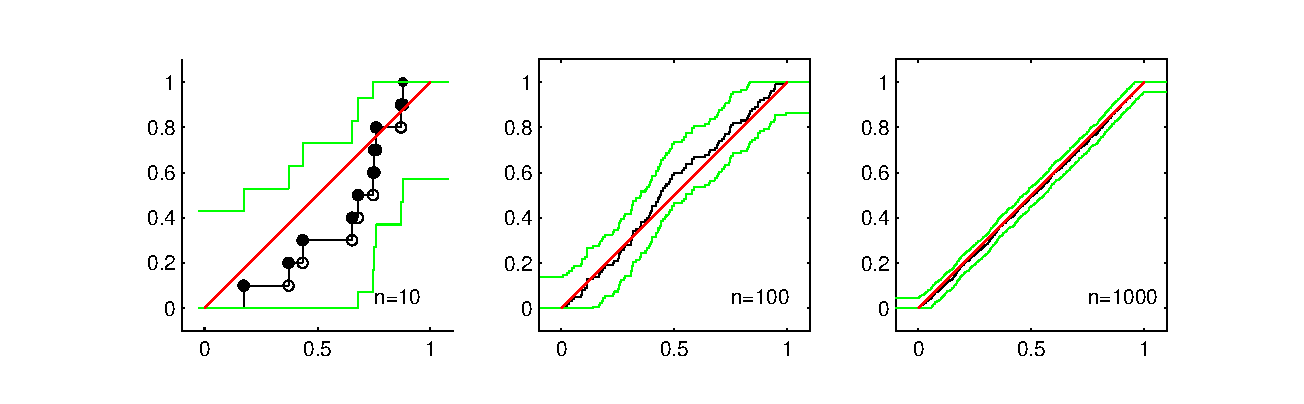
\includegraphics [width=5.5in]{figures/UniformECDFsBands}}
\end{figure}
\end{labwork}
Next we look at a more interesting example involving real-world data.
\begin{labwork}[Non-parametric Estimation of the DF of Times Between Earth Quakes]\label{LW:NZSIEQTimesECDFsConfBands}
Suppose that the $6,128$ observed times between Earth quakes in  NZ between 18-Jan-2008 02:23:44 and 18-Aug-2008 19:29:29 are:
$$X_1,\ldots,X_{6128} \overset{IID}{\sim} F^*, \qquad F^* \in \{ \text{all DFs} \} \enspace .$$
Then the non-parametric point estimate of the unknown $F^*$ is $\widehat{F}_{6128}$, the ECDF of the inter earth quake times.  We plot the non-parametric point estimate as well as the 95\% confidence bands for $F^*$ in  \hyperref[F:NZSIEQTimesECDFsConfBands]{Figure~\ref*{F:NZSIEQTimesECDFsConfBands}}.
\begin{figure}[htpb]
\caption{The empirical DF $\widehat{F}_{6128}$ for the inter earth quake times and the $95\%$ confidence bands for the non-parametric experiment.  \label{F:NZSIEQTimesECDFsConfBands}}
\centering   \makebox{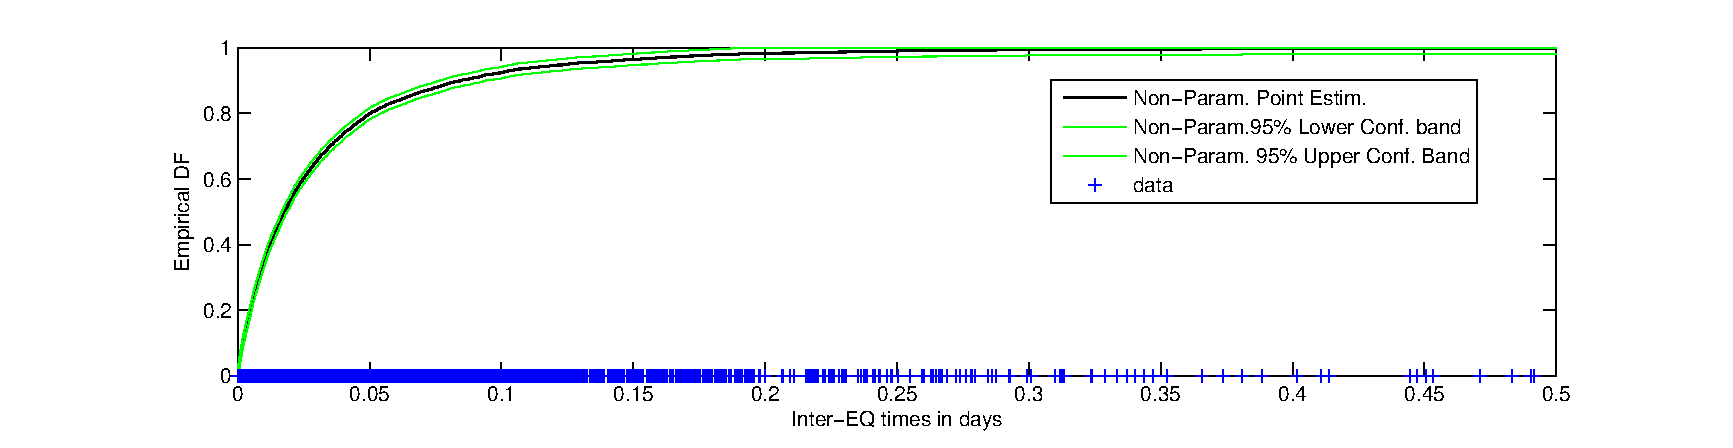
\includegraphics[width=6.5in]{figures/NZSIEQTimesECDFsConfBands}}
\end{figure}
\VrbMf[label=NZSIEQTimesECDFsConfBands.m]{scripts/NZSIEQTimesECDFsConfBands.m}
\end{labwork}

Recall the poor fit of the Exponential PDF at the MLE for the Orbiter waiting time data.  We can attribute the poor fit to coarse resolution of the waiting time measurements in minutes and the rigid decaying form of the exponential PDFs.  Let us revisit the Orbiter waiting time problem with our non-parametric estimator.  

\begin{labwork}[Non-parametric Estimation of Orbiter Waiting Times DF]\label{LW:OrbiterECDFsConfBands}
Suppose that the waiting times at the Orbiter bus stop are:
$$X_1,\ldots,X_{132} \overset{IID}{\sim} F^*, \qquad F^* \in \{ \text{all DFs} \} \enspace .$$
Then the non-parametric point estimate of $F^*$ is $\widehat{F}_{132}$, the ECDF of the $132$ Orbiter waiting times.
\begin{figure}[htpb]
\caption{The empirical DF $\widehat{F}_{132}$ for the Orbiter waiting times and the $95\%$ confidence bands for the non-parametric experiment.  \label{F:OrbiterECDFsConfBands}}
\centering   \makebox{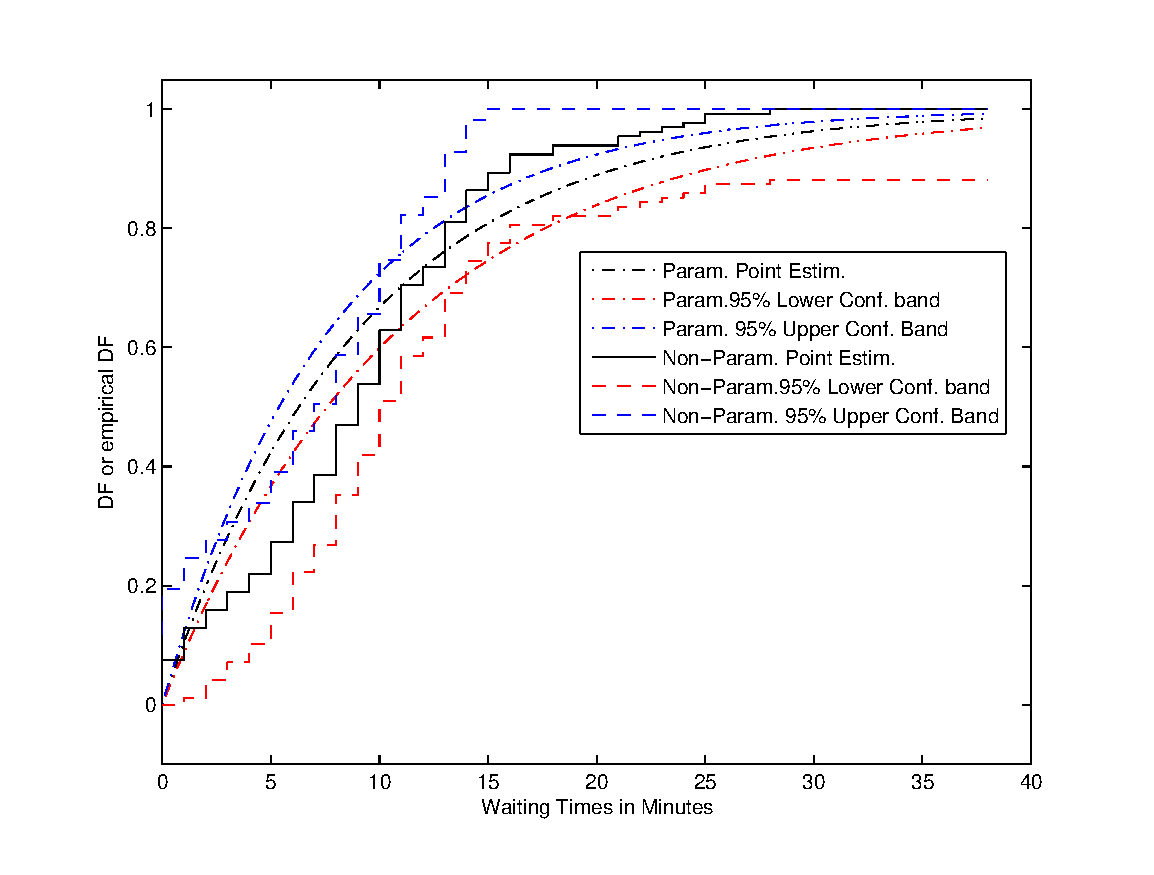
\includegraphics[width=5.5in]{figures/OrbiterECDFsConfBands}}
\end{figure}
We compute and plot the non-parametric point estimate as well as the 95\% confidence bands for the unknown DF $F^*$ beside the parametric estimate and $95\%$ confidence bands from \hyperref[LW:ExponentialMLECIOrbiter]{Labwork~\ref*{LW:ExponentialMLECIOrbiter}}.  Clearly, the non-parametric estimate is preferable to the parametric one for this example.  Notice how the non-parametric confidence bands do not contain the parametric estimate of the DF. 
\VrbMf[label=OrbiterECDFsConfBands.m]{scripts/OrbiterECDFsConfBands.m}
\end{labwork}


\begin{example}
First take a look at \hyperref[DA:WebLogs]{Data~\ref*{DA:WebLogs}} to understand how the web login times to our Maths \& Stats Department's web server (or requests to our WWW server) were generated. \hyperref[F:WebLogTimesECDFs]{Figure~\ref*{F:WebLogTimesECDFs}} shows the login times in units of seconds over a 24 hour period starting at 0357 hours and 30 seconds (just before 4:00AM) on October 1st, 2007 (red line) and on October 2nd, 2007 (magenta). 
\begin{figure}[htpb]
\caption{The empirical DFs $\widehat{F}^{(1)}_{n_1}$ with $n_1= 56485$, for the web log times starting October 1, and $\widehat{F}^{(2)}_{n_2}$ with $n_2=53966 $, for the web log times starting October 2.  Their $95\%$ confidence bands are indicated by the green.  \label{F:WebLogTimesECDFs}}
\centering   \makebox{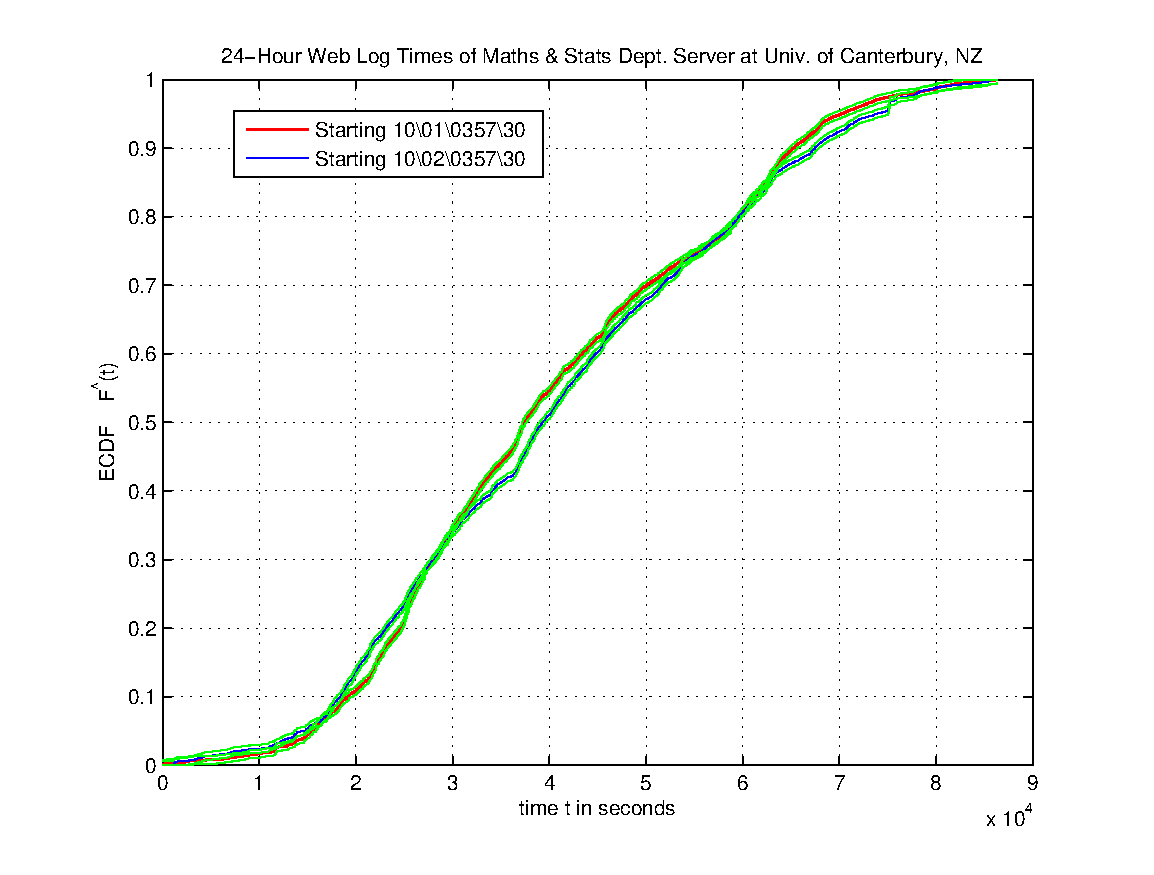
\includegraphics [width=4.5in]{figures/WebLogTimesECDFsBands}}
%WebLogTimesECDFs.eps}}
\end{figure}
If we assume that some fixed and unknown DF $F^{(1)}$ specifies the distribution of login times for October 1st data and another DF $F^{(2)}$ for October 2nd data, then the non-parametric point estimates of  $F^{(1)}$ and $F^{(2)}$ are simply the empirical DFs $\widehat{F}^{(1)}_{n_1}$ with $n_1= 56485$ and $\widehat{F}^{(2)}_{n_2}$ with $n_2=53966 $, respectively, as depicted in  \hyperref[F:WebLogTimesECDFs]{Figure~\ref*{F:WebLogTimesECDFs}}.  See the script of {\tt WebLogDataProc.m} in \hyperref[DA:WebLogs]{Data~\ref*{DA:WebLogs}} to appreciate how the ECDF plots in \hyperref[F:WebLogTimesECDFs]{Figure~\ref*{F:WebLogTimesECDFs}} were made.
\end{example}

\section{Plug-in Estimators of Statistical Functionals}\label{S:PlugIn}
Recall from \hyperref[S:Statistics]{Chapter~\ref*{S:Statistics}} that a {\bf statistical functional} is simply any function of the DF $F$.  For example, the median $T(F) = F^{[-1]}(1/2)$ is a statistical functional.  Thus, $T(F): \{ \text{All DFs }\} \to \Tz$, being a map or function from the space of DFs to its range $\Tz$, is a functional. 
The idea behind the plug-in estimator for a statistical functional is simple: just plug-in the point estimate $\widehat{F}_n$ instead of the unknown DF $F^*$ to estimate the statistical functional of interest.
\begin{definition}[Plug-in estimator]
Suppose, $X_1,\ldots,X_n \overset{IID}{\sim} F^*$.  The plug-in estimator of a statistical functional of interest, namely, $T(F^*)$, is defined by:
\[
\widehat{T}_n := \widehat{T}_n (X_1,\ldots,X_n) = T(\widehat{F}_n) \ .
\]
\end{definition}

\begin{definition}[Linear functional]
If $T(F) = \int r(x) dF(x)$ for some function $r(x):\Xz\to \Rz$, then $T$ is called a {\bf linear functional}.  Thus, $T$ is linear in its arguments:
\[
T(a F + a' F') = a T(F) + a' T(F') \enspace .
\]
\end{definition}

\begin{prop}[Plug-in Estimator of a linear functional]
The plug-in estimator for a linear functional $T = \int r(x) dF(x)$ is:
\[
\boxed{
T(\widehat{F}_n) = \int r(x) d \widehat{F}_n(x)=\frac{1}{n}\sum_{i=1}^n r(X_i) 
} \enspace .
\]
\end{prop}

Some specific examples of statistical linear functionals we have already seen include:
\begin{enumerate}
\item The {\bf mean} of RV $X \sim F$ is a function of the DF $F$:  
\[
T(F) = \e(X) = \int x\,dF(x) \ .
\]
\item The {\bf variance} of RV $X \sim F$ is a function of the DF $F$:  
\[
T(F) = \e(X-\e(X))^2 = \int (x-\e(X))^2\,dF(x) \ .
\]
\item The {\bf value of DF at a given $x \in \Rz$} of RV $X \sim F$ is also a function of DF $F$:
\[
T(F) = F(x) \  .
\]
\item The {\bf $q^{\text{th}}$ quantile} of RV $X \sim F$: 
\[
T(F) = F^{[-1]}(q) \ \text{ where } q \in [0,1] \ .
\]
\item The {\bf first quartile} or the {\bf $0.25^{\text{th}}$ quantile} of the RV $X \sim F$: 
\[
T(F) = F^{[-1]}(0.25) \ .
\]
\item The {\bf median} or the {\bf second quartile} or the {\bf $0.50^{\text{th}}$ quantile} of the RV $X \sim F$: 
\[
T(F) = F^{[-1]}(0.50) \  .
\]
\item The {\bf third quartile} or the {\bf $0.75^{\text{th}}$ quantile} of the RV $X \sim F$: 
\[
T(F) = F^{[-1]}(0.75) \ .
\]
\end{enumerate}


\begin{labwork}[Plug-in Estimate for Median of Web Login Data]
Compute the plug-in estimates for the median for each of the data arrays:
\[
\text{{\tt WebLogSeconds20071001035730} and {\tt WebLogSeconds20071002035730} }
\]
that can be loaded into memory by following the commands in the first $13$ lines of the script file {\tt WebLogDataProc.m} of \hyperref[DA:WebLogs]{Data~\ref*{DA:WebLogs}}.
\end{labwork}

\begin{labwork}[Plug-in Estimates of Times Between Earth Quakes]\label{LW:PlugInEstimatesEarthQuakes}
Compute the plug-in estimates for the median and mean time in minutes between earth quakes in NZ using the data in {\tt earthquakes.csv}. 
\VrbMf[label=NZSIEQTimesPlugInEstimates.m]{scripts/NZSIEQTimesPlugInEstimates.m}
\begin{VrbM}
>> NZSIEQTimesPlugInEstimates
PlugInMedianEstimate =    0.0177
PlugInMedianEstimateMinutes =   25.5092
PlugInMeanEstimate =    0.0349
PlugInMeanEstimateMinutes =   50.2278
\end{VrbM}
\end{labwork}

Note that any statistical functional can be estimated using the plug-in estimator.  However, to produce a $1-\alpha$ confidence set for the plug-in point estimate, we need bootstrap methods.  The subject of next chapter.

